\begin{frame}[t, c]{Chaotic thermosyphon}{Characterizing its dynamics}
  \centering
  \movie[width=.8\textwidth, autostart, loop]{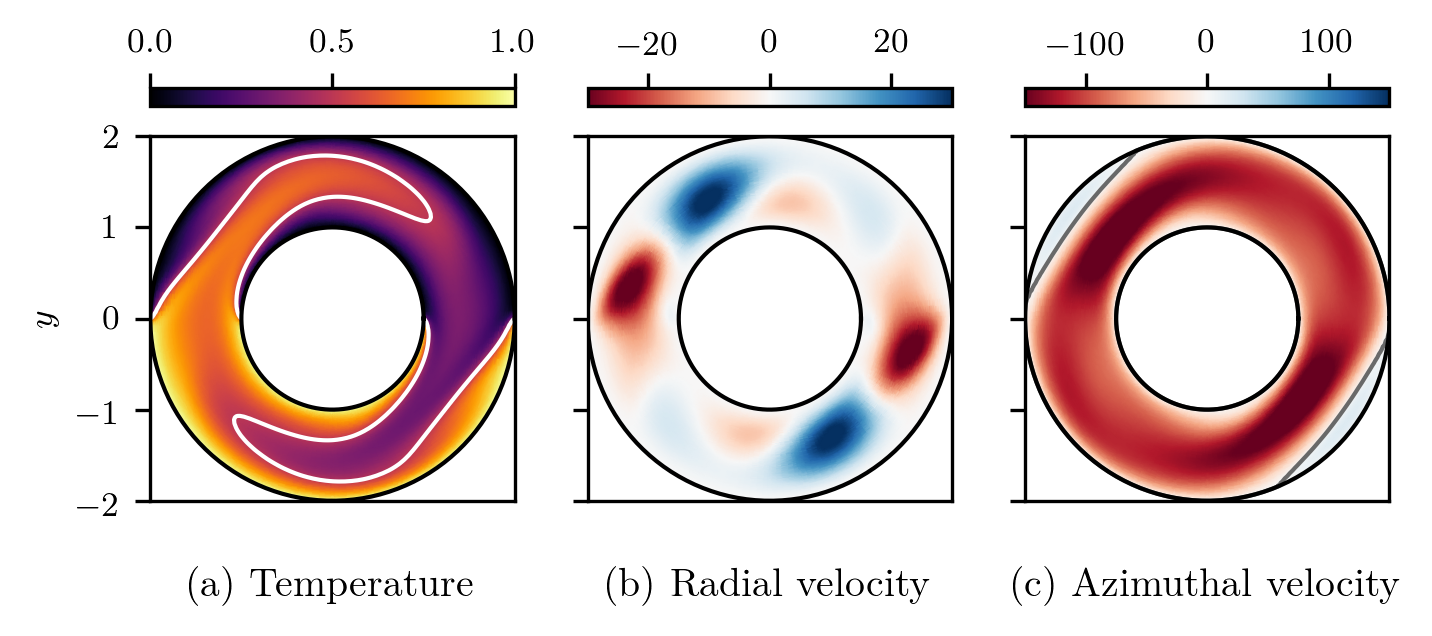
\includegraphics[width=.8\textwidth]{chaotic_thermosyphon_00000}}{imgs/chaotic_thermosyphon.mp4}

  \vspace{1cm}
\end{frame}

% \begin{frame}[t, c]{Chaotic thermosyphon}{Characterizing its dynamics}
%   \begin{minipage}{.48\textwidth}
%     \begin{itemize}
%       \item Mean flow and fluctuations are symmetric w.r.t.\ the vertical axis.
%
%       \medskip
%
%       \item Temperature fluctuations are localized close to the discontinuity at the walls.
%
%       \medskip
%
%       \item Azimuthal velocity is relatively invariant in the azimuthal direction.
%     \end{itemize}
%   \end{minipage}%
%   \hfill
%   \begin{minipage}{.48\textwidth}
%     \centering
%     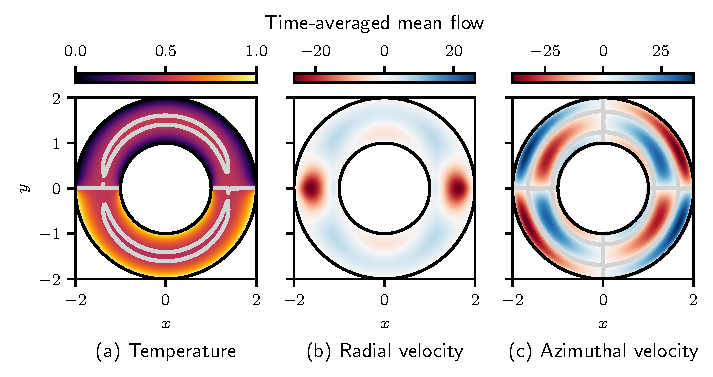
\includegraphics[width=.9\textwidth]{mean_flow} \\
%     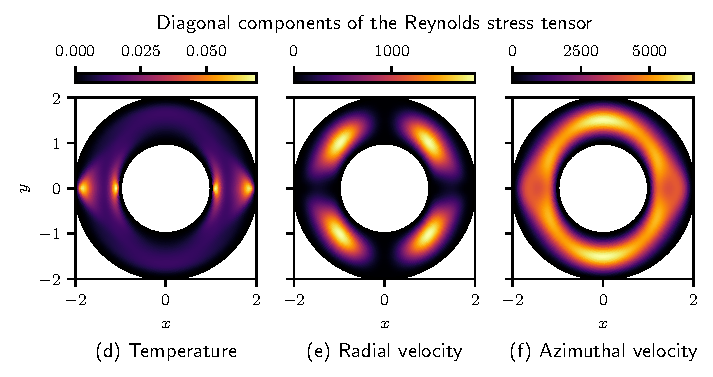
\includegraphics[width=.9\textwidth]{reynolds_stresses}
%   \end{minipage}
%
%   \vspace{1cm}
% \end{frame}

\begin{frame}[t, c]{Chaotic thermosyphon}{Characterizing its dynamics}
  \begin{minipage}{.58\textwidth}
    \begin{figure}
      \subfigure[Flow rate \( m(t) \)]{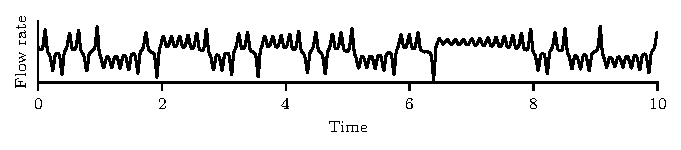
\includegraphics[width=\textwidth]{flow_rate_time_series}} \\
      \subfigure[Empirical PDF]{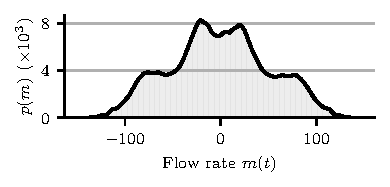
\includegraphics[width=.48\textwidth]{flow_rate_empirical_pdf}}%
      \hfill
      \subfigure[PSD of \( \dot{m}(t) \)]{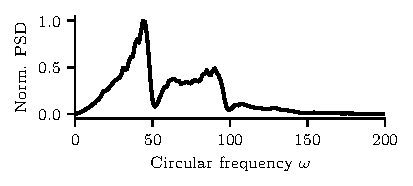
\includegraphics[width=.48\textwidth]{flow_rate_psd}}
    \end{figure}
  \end{minipage}%
  \hfill
  \begin{minipage}{.38\textwidth}
    \begin{itemize}
    \item Clockwise and counter-clockwise rotations are equally likely.

      \medskip
      
    \item Dominant time-scale associated w/ the oscillation in one direction.
      
      \medskip
      
    \item Continuous spectrum due to the chaotic nature of the system.
    \end{itemize}
  \end{minipage}

  \vspace{1cm}
\end{frame}

\begin{frame}[t, c]{Chaotic thermosyphon}{Characterizing its dynamics}
  \vspace{-0.5cm}
  % \begin{minipage}{.38\textwidth}
  %   \begin{itemize}
  %     \item Correlation decay due to the switches.

  %     \medskip

  %     \item Most of the time, a single oscillation occurs before switching.

  %     \medskip

  %     \item Behaviour very similar to that of the Lorenz system.
  %   \end{itemize}
  % \end{minipage}%
  % \hfill
  % \begin{minipage}{.58\textwidth}
    \begin{figure}
      \subfigure[Flow rate \( m(t) \)]{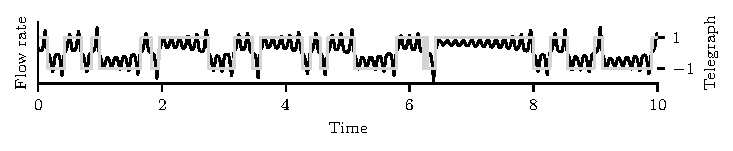
\includegraphics[width=.8\textwidth]{flow_rate_telegraph_signal}} \\
      \subfigure[Autocorr.\ function]{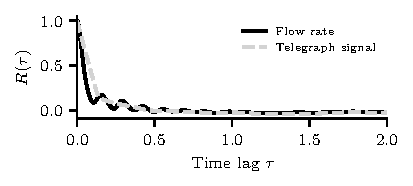
\includegraphics[width=.4\textwidth]{flow_rate_autocorrelation}}%
      %\hfill
      \subfigure[Time-scale dist.]{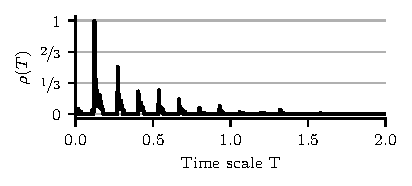
\includegraphics[width=.4\textwidth]{flow_rate_time_scale_distribution}}
    \end{figure}
  % \end{minipage}

  \vspace{2cm}
\end{frame}

% \begin{frame}[t, c]{Chaotic thermosyphon}{Connection with Lorenz system}
%   \begin{minipage}{.48\textwidth}
%     \begin{figure}
%       \centering
%       \subfigure[Lorenz time series]{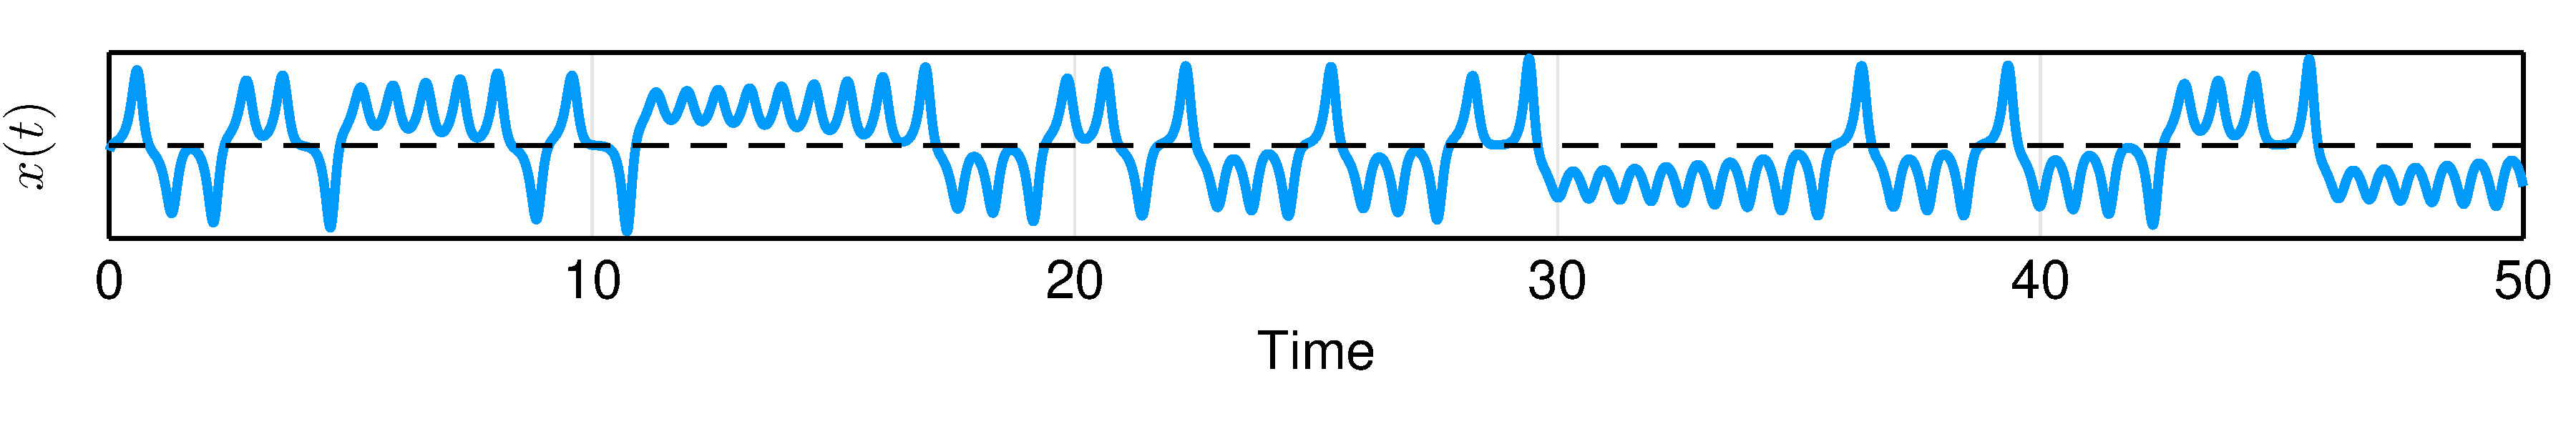
\includegraphics[width=\textwidth]{lorenz_time_series}} \\
%       \subfigure[Attractor reconstruction]{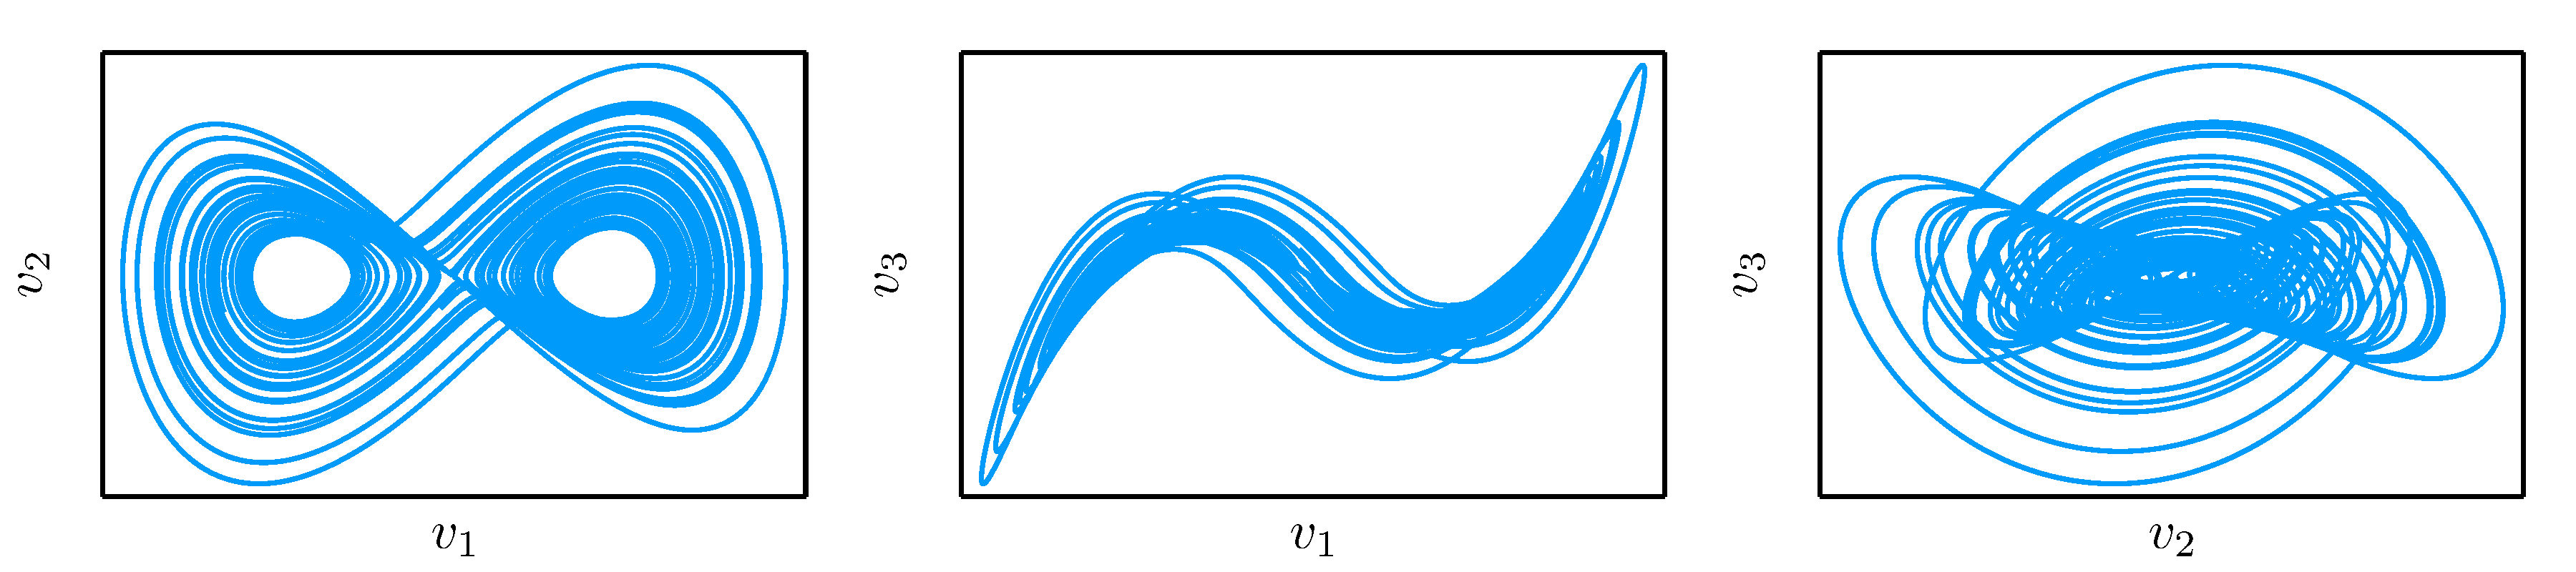
\includegraphics[width=\textwidth]{lorenz_broomhead_king_reconstruction}} \\
%       \subfigure[Poincaré section]{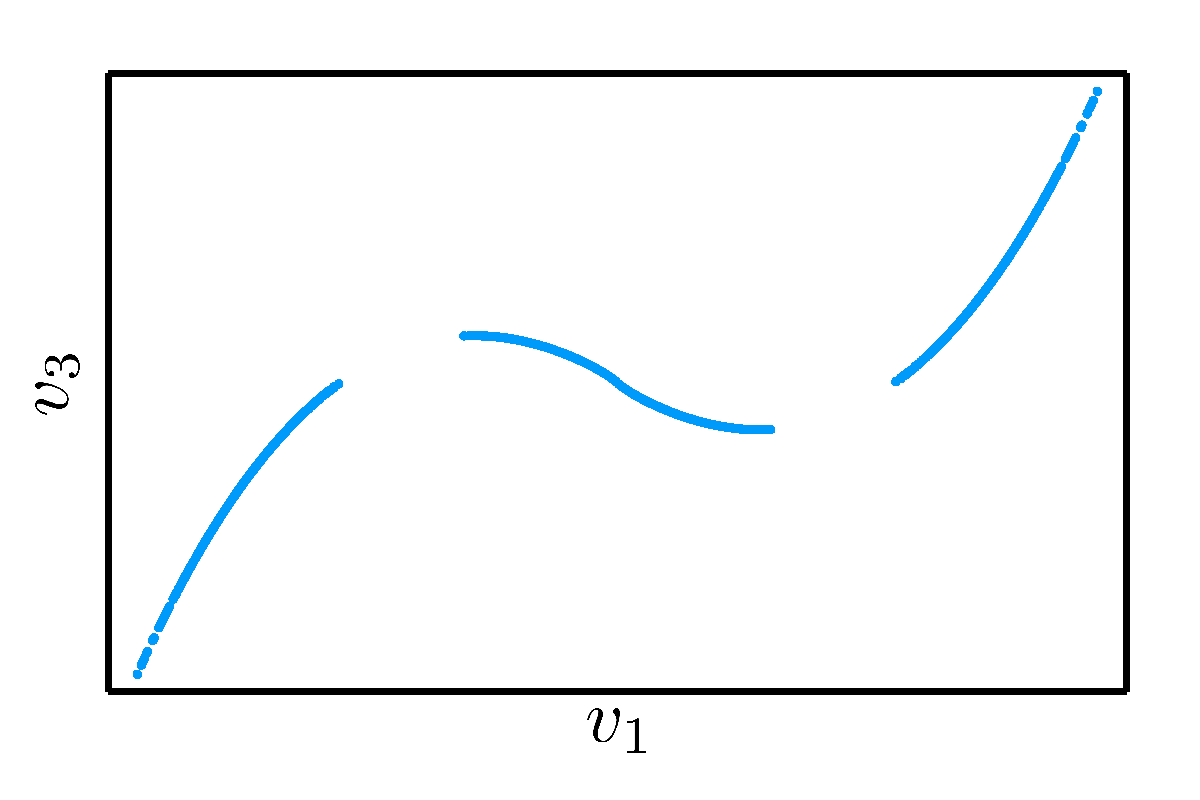
\includegraphics[width=.3333\textwidth]{lorenz_poincare_section}}
%     \end{figure}
%   \end{minipage}%
%   \hfill
%   \begin{minipage}{.48\textwidth}
%     \begin{figure}
%       \centering
%       \subfigure[Flow rate time series]{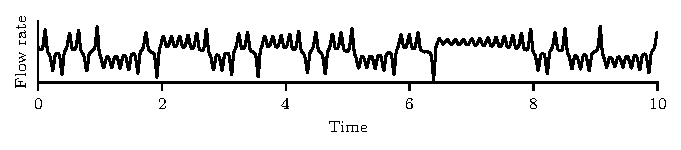
\includegraphics[width=\textwidth]{flow_rate_time_series}} \\
%       \subfigure[Attractor reconstruction]{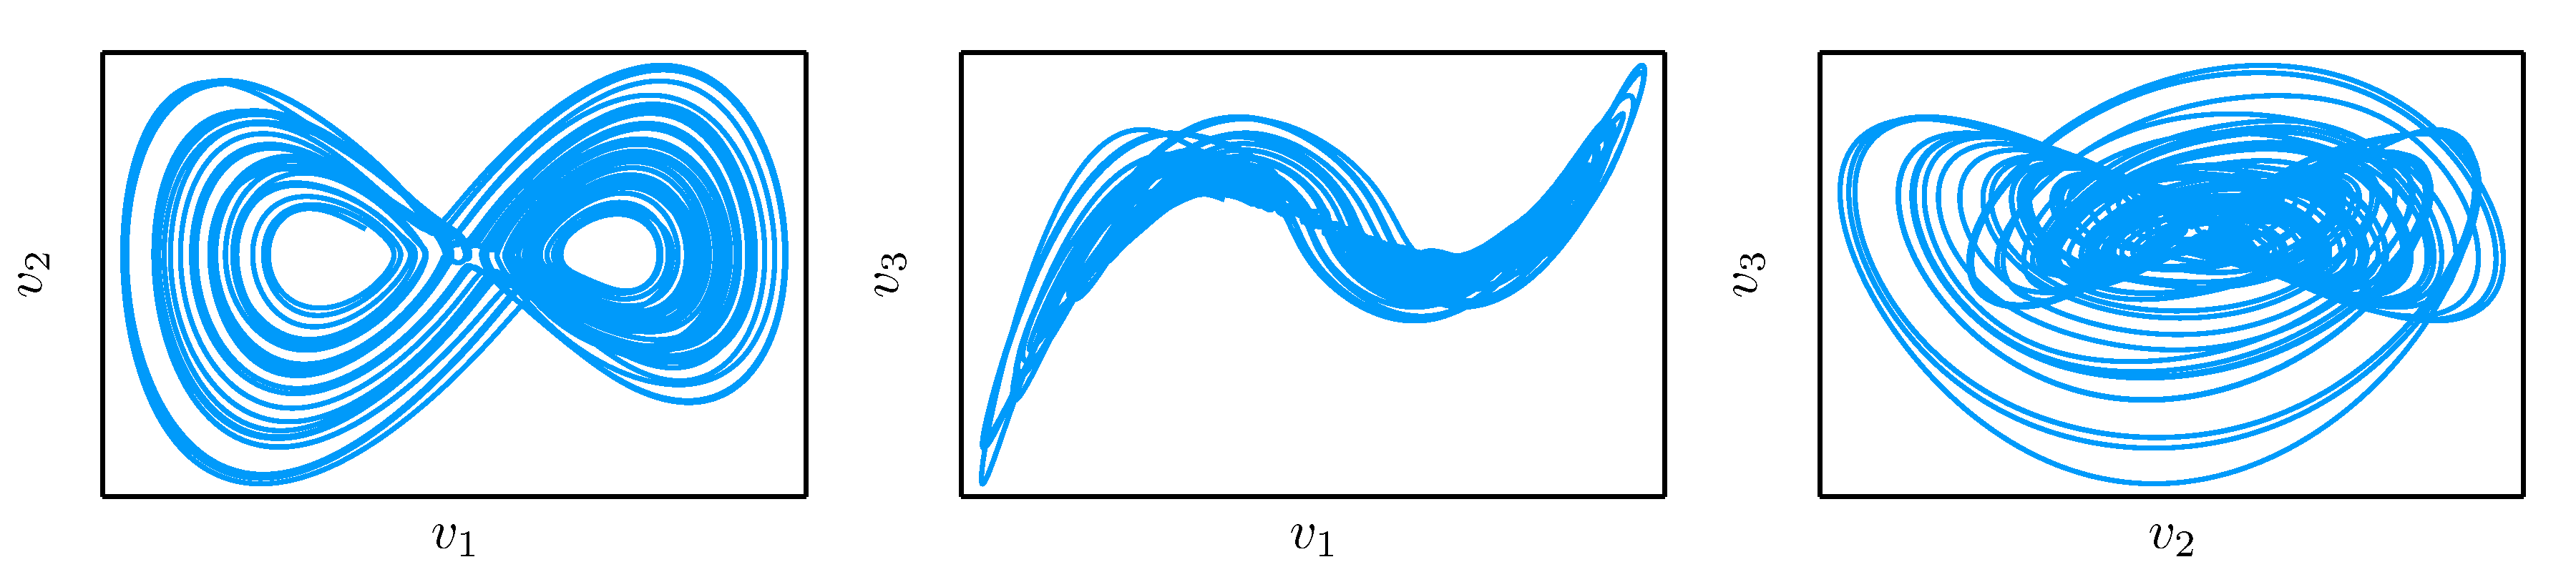
\includegraphics[width=\textwidth]{broomhead_king_reconstruction}} \\
%       \subfigure[Poincaré section]{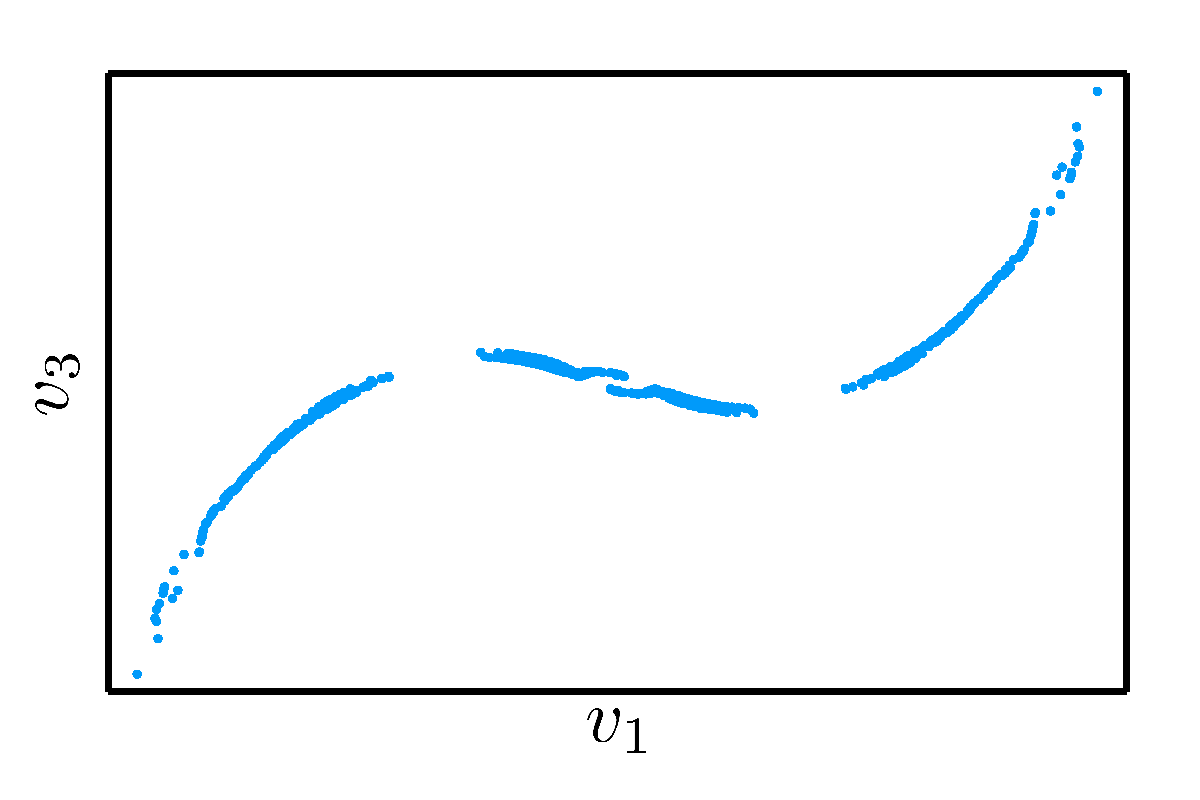
\includegraphics[width=.3333\textwidth]{flow_rate_poincare_section}}
%     \end{figure}
%   \end{minipage}
%
%   \vspace{1cm}
% \end{frame}
